\documentclass[aspectratio=169]{beamer}
\usetheme{metropolis}           % Use metropolis theme
\title{Machine learning im Bereich der Robotik}
\date{\today}
\author{Robin Eberhard}

\begin{document}
  \maketitle
  \begin{frame}{Pancakes machen}
  \begin{center}
  	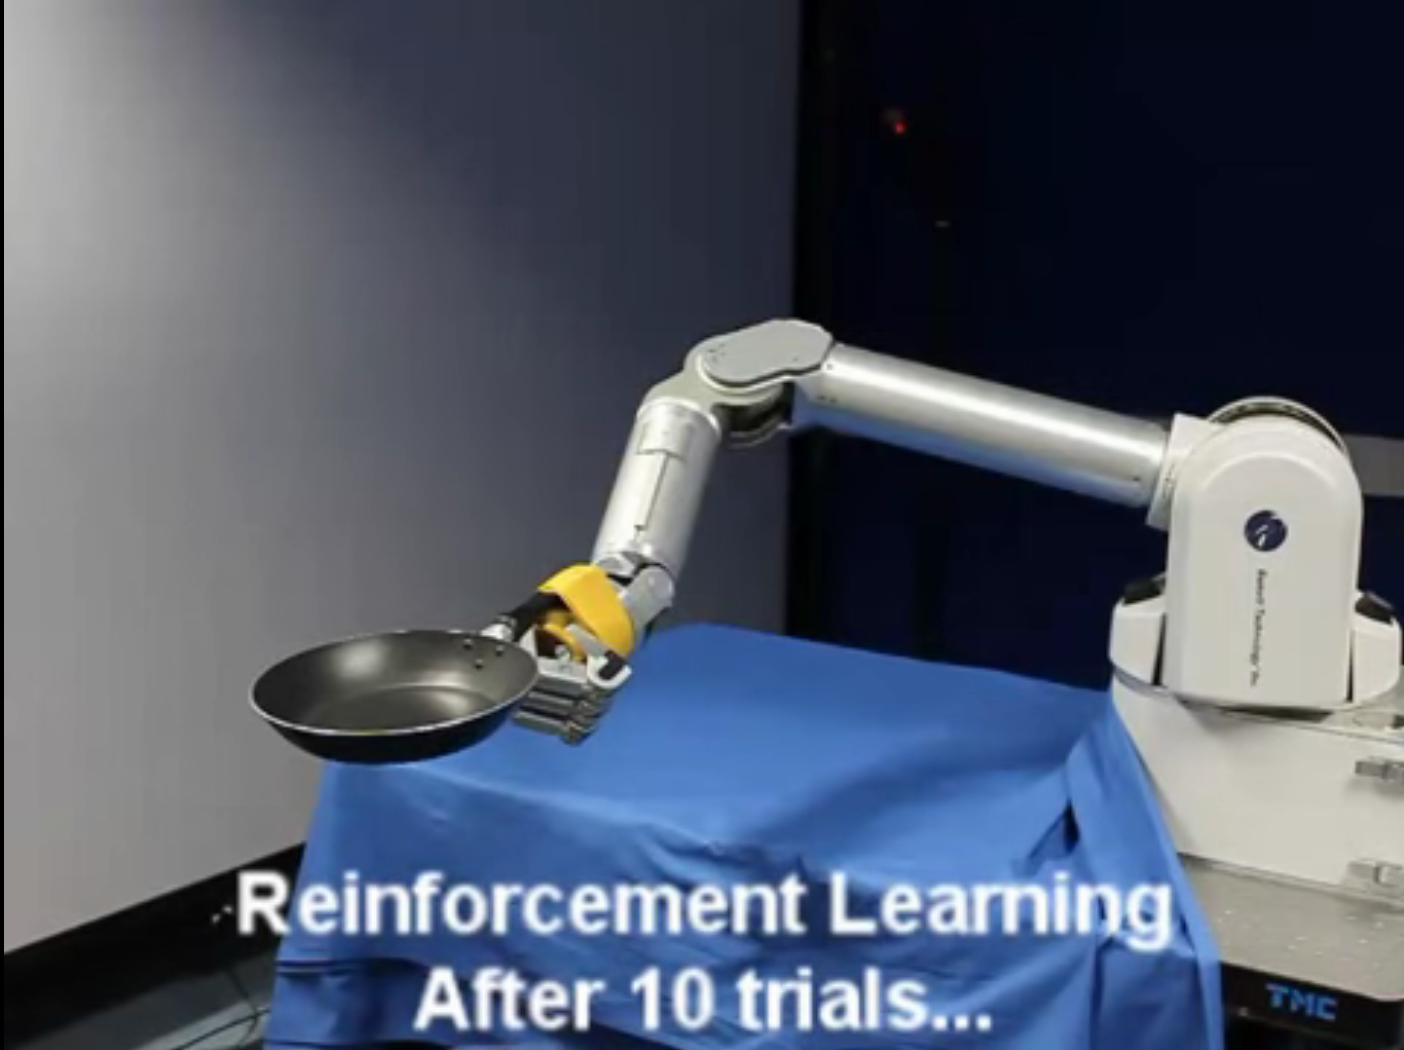
\includegraphics[scale=0.15]{img/pancake.png} \\
  	\url{https://youtu.be/W_gxLKSsSIE?t=51}
  \end{center}
  \end{frame}
  
  %%%%%%%%%%%%%%%%%%%%%%%%%%%%%%%%%%%%%%%%%%%%%%%%
  %%%%%%%%% Quadrotor %%%%%%%%%%%%%%%%%%%%%%%%%%%%
  \section{Quadrotor im Wald}
  \begin{frame}{Quadrotor im Wald}
  \begin{center}
  	% http://rpg.ifi.uzh.ch/docs/RAL16_Giusti.pdf
  	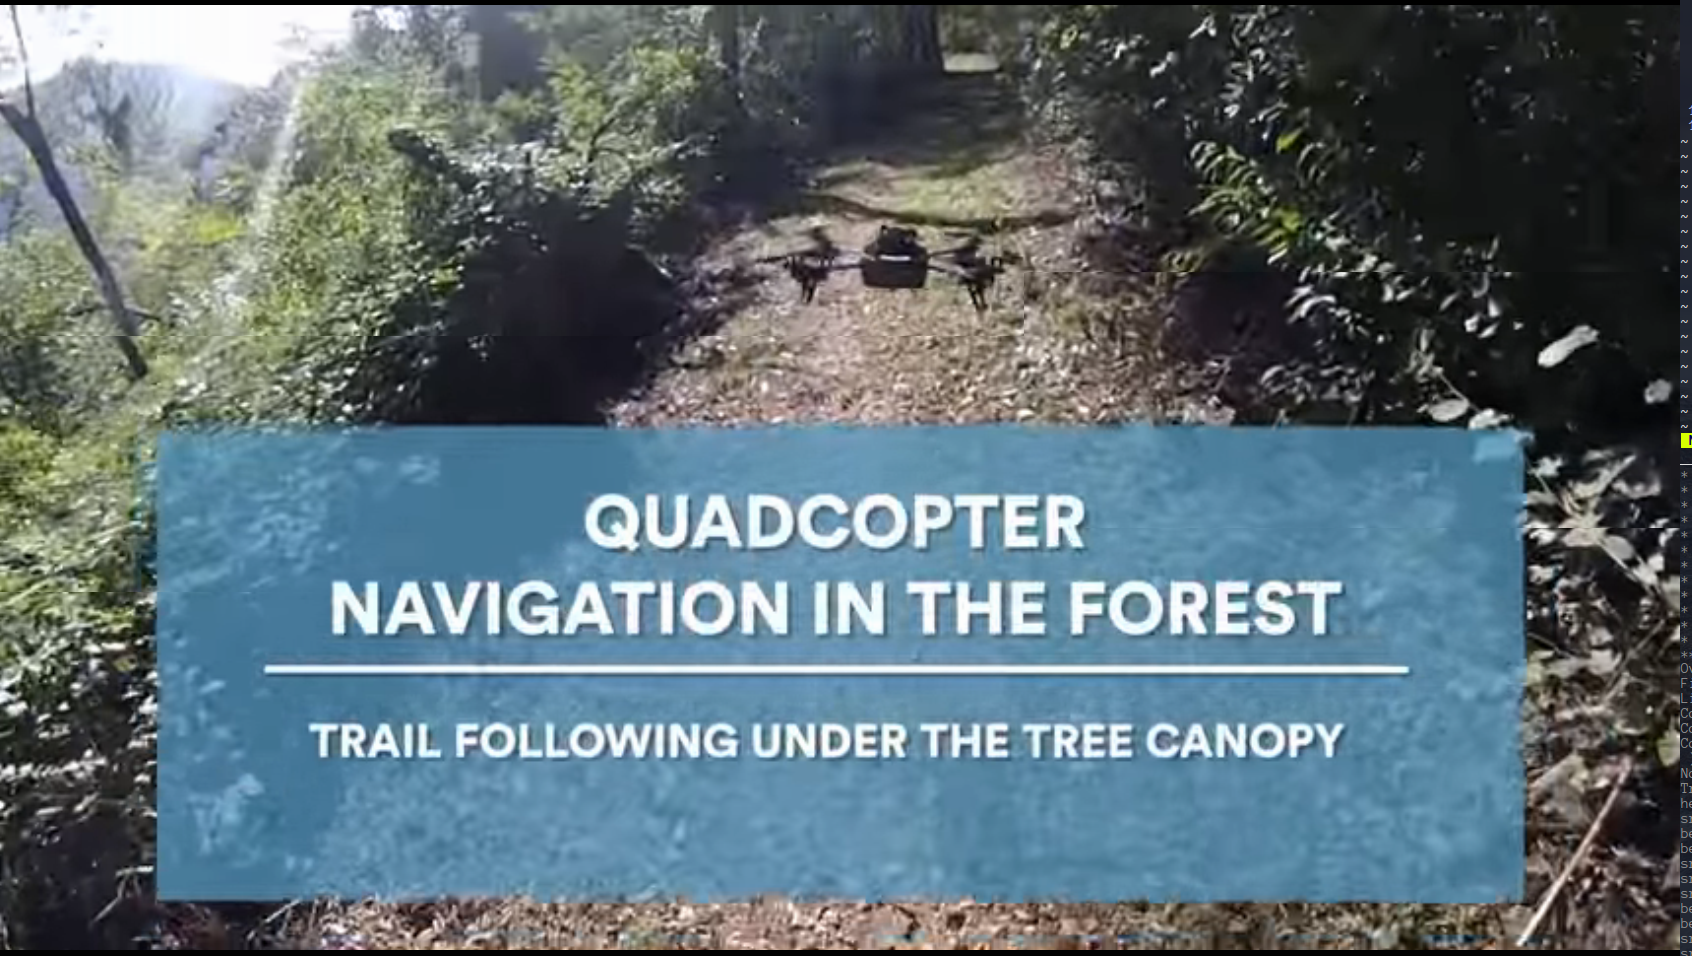
\includegraphics[scale=0.15]{img/quadrotor.png} \\
  	\url{https://www.youtube.com/watch?v=umRdt3zGgpU}
  \end{center}
  \end{frame}
  
  \begin{frame}{Quadrotor im Wald}
  Methodik
  	\begin{itemize}
  		\item Computer Vision
  		\item Deep Neural Network
  		\item Supervised learning
  	\end{itemize}
  \end{frame}
  
  \begin{frame}{Quadrotor im Wald}
  Funktionsweise
  	\begin{itemize}
  		\item Phase 1: Aufnahme des Trails
  		\begin{itemize}
  			\item Drei Kameras um 30° versetzt
  			\item Mittlere Kamera in Richtung des Pfads
  			\item Kategorisierung der Kameras als Links, Mitte und Rechts
  		\end{itemize}
  		\pause
  		\item Phase 2: Das System trainieren
  		\begin{itemize}
  			\item Das System erhält >17.000 Trainingsbilder
  			\item Das System versucht diese in Links, Mitte und Rechts zu kategorisieren
  		\end{itemize}
  		\pause
  		\item Phase 3: Das System testen
  		\begin{itemize}
  			\item Das System wird zuerst mit >7000 Testbildern getestet
  			\item Später: Test auf echten Trails
  		\end{itemize}
  	\end{itemize}
  \end{frame}
  
  \begin{frame}{Quadrotor im Wald}
  	Zusammenfassung
  	\begin{itemize}
  		\item Bei der Kategorisierung ist die Drone stellenweise besser als Menschen
  		\pause
  		\item Die Drone schafft es selbstständig auch auf unbekannten Wegen zu fliegen
  		
  	\end{itemize}
  \end{frame}
  
  %%%%%%%%%%%%%%%%%%%%%%%%%%%%%%%%%%%%%%%%%%%%%%%%
  %%%%%%%%% EUROPA2 %%%%%%%%%%%%%%%%%%%%%%%%%%%%%%
  \section{EUROPA2 - European Robotic Pedestrian Assistant 2.0}
  \begin{frame}{EUROPA2 - European Robotic Pedestrian Assistant 2.0}
  	\begin{center}
  		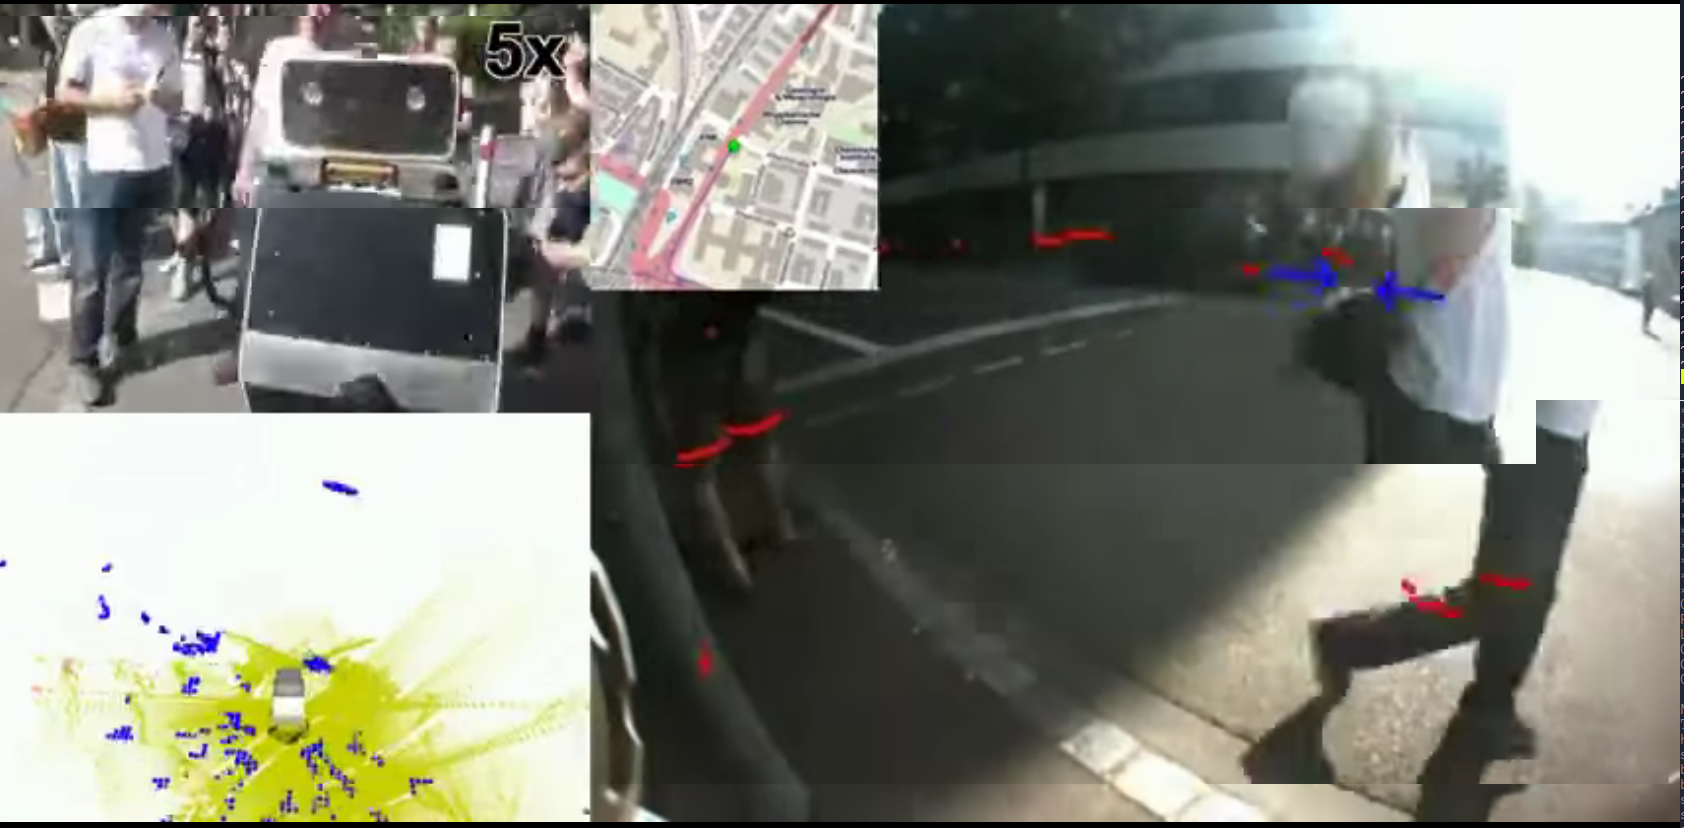
\includegraphics[scale=0.15]{img/europa.png} \\
  		\url{https://youtu.be/A9A29wpkTaU?t=246}
  	\end{center}
  \end{frame}
  
  \begin{frame}{EUROPA2 - European Robotic Pedestrian Assistant 2.0}
  	\begin{center}
  		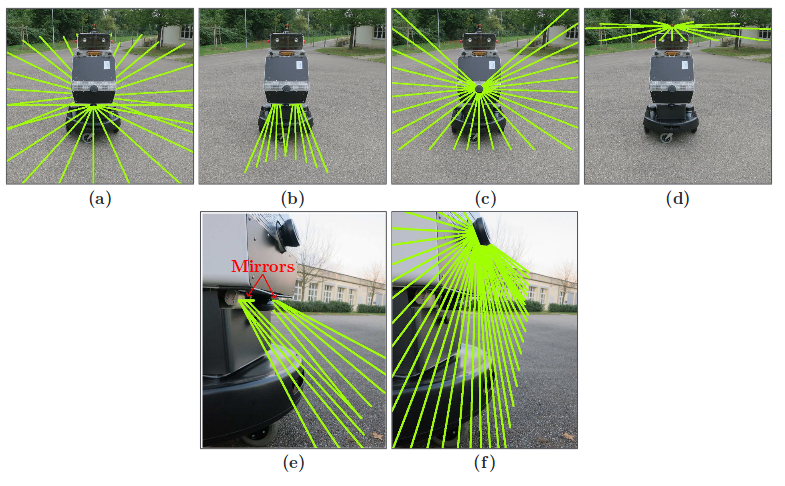
\includegraphics[scale=0.38]{img/europa2_lasers.png}
  	\end{center}
  \end{frame}
  
  \begin{frame}{EUROPA2 - European Robotic Pedestrian Assistant 2.0}
  	Es gibt ca 60 Dokumente zu Themen wie
  	\begin{itemize}
  		%\item \href{http://europa2.informatik.uni-freiburg.de/files/kretzschmar14icra.pdf}{\textit{Vorhersagen zur Bewegung von Menschen}}
  		%\pause
  		\item \href{http://europa2.informatik.uni-freiburg.de/files/ilg14icra.pdf}{Rekonstruktion von bewegten Objekten mithilfe eines 2D Laserscanners und einer Kamera}
  		\pause
  		\item \href{http://europa2.informatik.uni-freiburg.de/files/kuemmerle14jfr.pdf}{\textit{Autonome Navigation in populierten Gegenden}}
  		\pause
  		\item \href{http://europa2.informatik.uni-freiburg.de/files/ruchti15icra.pdf}{Lokalisierung in OpenStreetMap mithilfe eines 3D scanners}
  		\pause
  		%\item \href{http://europa2.informatik.uni-freiburg.de/files/vysotska15icra.pdf}{Lokalisierung unter verschiedenen Lichtverhältnissen}
  		\pause
  		\item \href{http://europa2.informatik.uni-freiburg.de/files/oliveira16icra.pdf}{\textbf{Identifizierung von menschlichen Körperteilen mithilfe von Computer Vision und Convoluted Neural Networks}}
  		\pause
  		\item \href{http://europa2.informatik.uni-freiburg.de/files/IROS16_1259_FI.pdf}{\textit{Vorhersage von menschlichen Aktionen}}
  		\pause
  		\item \href{http://europa2.informatik.uni-freiburg.de/files/kretzschmar16ijrr.pdf}{\textit{Lernen und Nachahmung von menschlichen Bewegungen}}
  	\end{itemize}
  \end{frame}
  
  %%%%%%%%%%%%%%%%%%%%%%%%%%%%%%%%%%%%%%%%%%%%%%%%
  %%%%%%%%% LifeNav %%%%%%%%%%%%%%%%%%%%%%%%%%%%%%
  \section{LifeNav}
  \begin{frame}{LifeNav}
  	\begin{center}
  		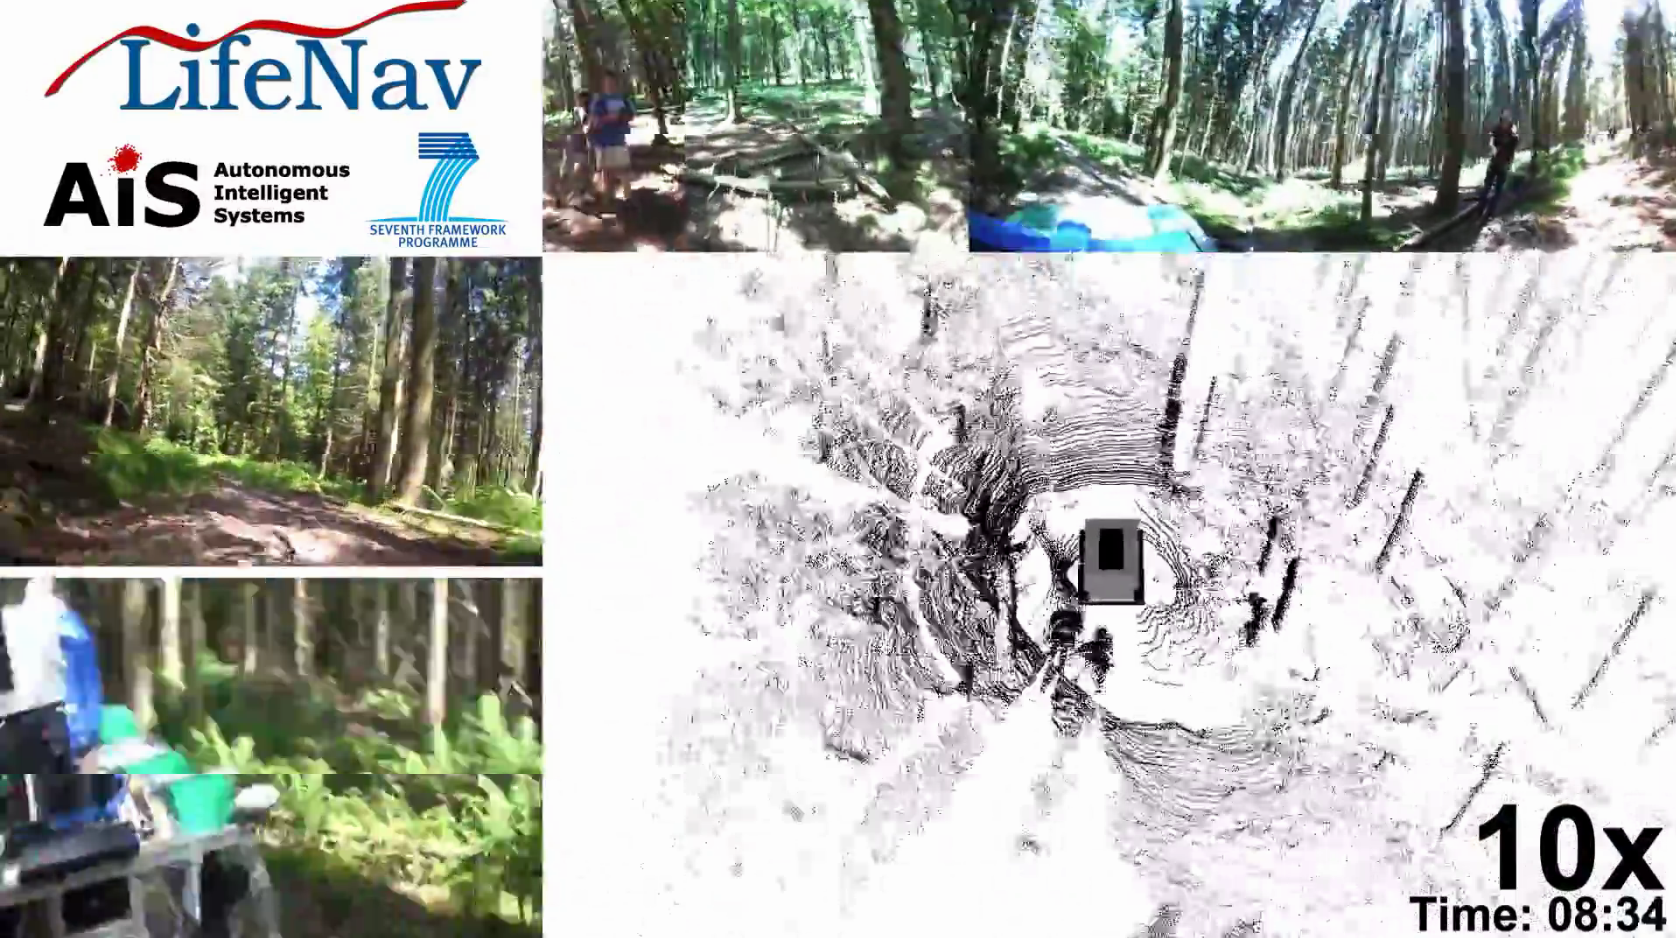
\includegraphics[scale=0.15]{img/lifenav.png} \\
  		\url{https://youtu.be/kdQUOZ7dPTc?t=7}
  	\end{center}
  \end{frame}
  
  \begin{frame}{LifeNav}
  	Es gibt ca 40 Dokumente zu Themen wie
  	\begin{itemize}
  		\item \href{http://www.lifelong-navigation.eu/files/tipaldi13icra.pdf}{Wiedererkennung von Orten}
  		\pause		
  		\item \href{http://www.lifelong-navigation.eu/files/tipaldi13ijrr.pdf}{Lokalisierung in veränderbaren Umgebungen}
  		\pause
  		\item \href{http://www.lifelong-navigation.eu/files/valada15isrr.pdf}{\textbf{Lernen von Features basierend auf Akkustik}}
  		\pause
  		\item \href{http://www.lifelong-navigation.eu/files/mazuran15icra.pdf}{\textit{Lehren und Optimierung eines Pfades}}
  		\pause
  		\item \href{http://www.lifelong-navigation.eu/files/valada16rssws.pdf}{\textbf{Segmentierung eines Bildes unter schwierigen Bedingungen}}
  	\end{itemize}
  \end{frame}
  
  \begin{frame}{LifeNav}
  	\begin{center}
  		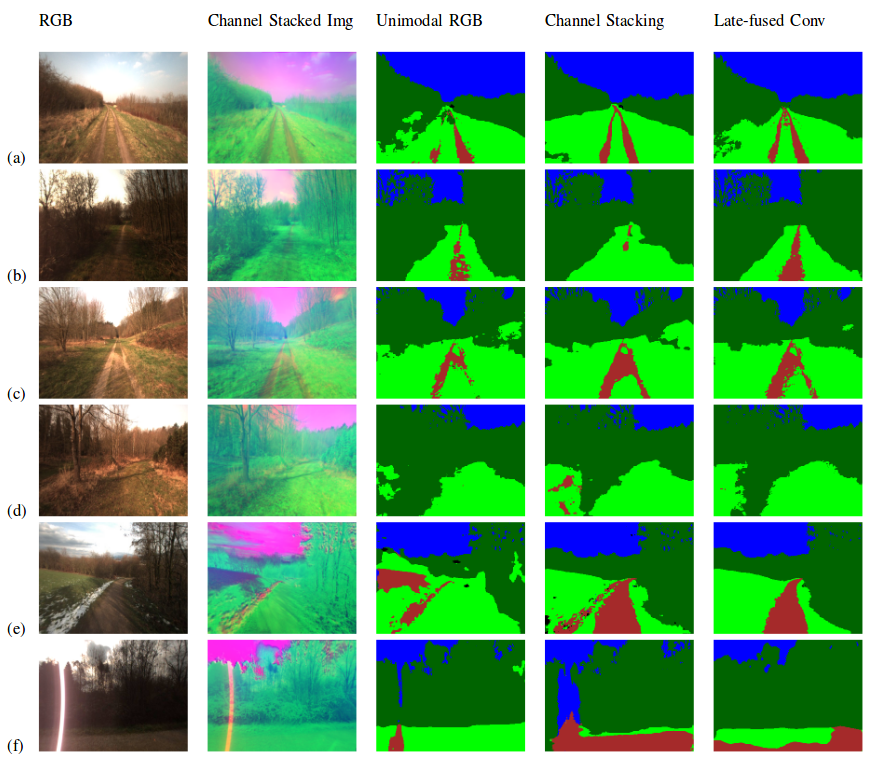
\includegraphics[scale=0.26]{img/segmentation.png}
  	\end{center}
  \end{frame}
  
  %%%%%%%%%%%%%%%%%%%%%%%%%%%%%%%%%%%%%%%%%%%%%%%%
  %%%%%%%%% Andere Projekte %%%%%%%%%%%%%%%%%%%%%%
  \section{Andere Projekte}
  \begin{frame}{Andere Projekte}
  	\begin{itemize}
  		% https://arxiv.org/pdf/1703.00420.pdf
  		% \item \href{https://youtu.be/9AOIwBYIBbs?t=70}{Bewegung ohne vorgegebene Karte}
  		% http://ieeexplore.ieee.org/stamp/stamp.jsp?arnumber=7605233
  		\item \href{https://www.youtube.com/watch?v=fL3YCIPxuhM&feature=youtu.be}{Jagen eines Beuteroboters}
  		% http://ieeexplore.ieee.org/stamp/stamp.jsp?arnumber=6630809
  		\item \href{https://youtu.be/hNsP6-K3Hn4?t=40}{Ausweichen von Hindernissen für fliegende Roboter}
  		% http://arxiv.org/pdf/1602.01783.pdf
  		\item Deepmind Bewegung ohne Lokalisierung \href{https://www.youtube.com/watch?v=nMR5mjCFZCw}{\underline{1}} \href{https://youtu.be/0xo1Ldx3L5Q}{\underline{2}}
  	\end{itemize}
  \end{frame}
  
\end{document}